\documentclass{../../oss-apphys-exam}

\renewcommand{\arraystretch}{1.5}
\usepackage{circuitikz} % to draw circuits!

\begin{document}
\genheader

\begin{center}
  \textbf{AP PHYSICS C CLASS 19: MAGNETISM, PART 3}
\end{center}
%\genfreedirections
  
\cpic{.5}{inout}

\begin{questions}
  % TAKEN FROM THE 2014 AP PHYSICS EXAM QUESTION E&M.2
  \question The rectangular loop of wire shown on the left in the figure above
  has mass $M$, length $L$, width $L/4$, and resistance $R$. It is initially
  moving to the right at constant speed $v_0$ , with no net force acting on
  it. At time $t=0$ the loop enters a region of length $2L$ that contains a
  uniform magnetic field of magnitude $B$ directed into the page. The loop
  emerges from the field at time $t_f$ with final speed $v_f$. Express all
  algebraic answers to the following in terms of $M$, $L$, $R$, $B$, $v_0$,
  and fundamental constants, as appropriate.
  \begin{parts}
    \part Let $x$ represent the position of the right end of the loop. Place a
    check mark in the appropriate box in each column in the table below to
    indicate whether the speed of the loop increases, decreases, or stays the
    same as the loop moves to the right.
    \uplevel{
      \centering
      \begin{tabular}{|c|c|c|c|c|}
        \hline
        & \multicolumn{4}{c|}{Position of Right End of Loop} \\ \hline
        Speed of Loop & $L<x<2L$ & $2L<x<3L$ & $3L<x<4L$ & $4L<x<5L$ \\
        \hline
        Increases & & & & \\
        \hline
        Dereases & & & & \\
        \hline
        Stays the Same & & & & \\
        \hline
      \end{tabular}
    }

    \part Derive an expression for the magnitude of the current induced in the
    loop as its right edge enters the field.
    \label{partb}
    \vspace{\stretch1}
    
    \part What is the direction of the induced current determined in part
    (\ref{partb})?

    \vspace{.15in}
    \underline{\hspace{.5in}} Clockwise\hspace{.6in}
    \underline{\hspace{.5in}} Counterclockwise

    \vspace{.15in} Justify your answer.
    \vspace{\stretch1}
    \newpage
    
    \part Write, but do not solve, a differential equation for the speed
    $v$ as a function of time as the loop enters the field.
    \vspace{\stretch1}
    
    \part What is the direction of the acceleration of the loop just before
    its left edge leaves the field?

    \vspace{.15in}
    \underline{\hspace{.5in}} Left\hspace{1in}
    \underline{\hspace{.5in}} Right\hspace{1in}
    \underline{\hspace{.5in}} Up\hspace{1in}
    \underline{\hspace{.5in}} Down
  \end{parts}
  
  \vspace{.15in}Justify your answer.
  \vspace{\stretch1}
  \newpage

  \uplevel{
    \centering
    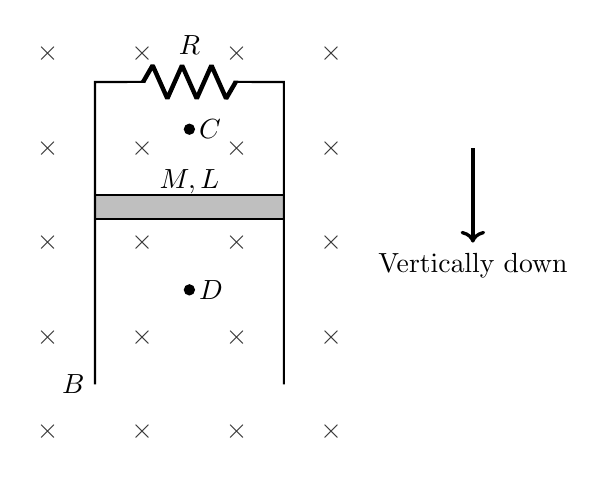
\begin{tikzpicture}[scale=1.2]
      \foreach \x in {0,...,3}{
        \foreach \y in {0,...,4}
        \node at (\x,\y){\textcolor{black!80}{$\times$}};
      }
      \draw[thick,fill=lightgray](.5,2.25) rectangle(2.5,2.5)
      node[above=1,midway]{$M,L$};
      \draw[thick](.5,.5)--(.5,3.7) node[pos=0,left]{$B$}
      to[R,l=$R$](2.5,3.7)--(2.5,.5);
      \fill (1.5,1.5) circle(.06) node[right]{$D$};
      \fill (1.5,3.2) circle(.06) node[right]{$C$};
      \draw[very thick,->](4.5,3)--(4.5,2) node[below]{Vertically down};
    \end{tikzpicture}
  }
  \question A conducting bar of mass $M$, length $L$, and negligible resistance
  is connected to two long vertical conducting rails of negligible resistance.
  The two rails are connected by a resistor of resistance $R$ at the top. The
  entire apparatus is located in a magnetic field of magnitude $B$ directed
  into the page, as shown in the figure above. The bar is released from rest
  and slides without friction down the rails.
  \begin{parts}
    \part What is the direction of the current in the resistor?
    
    \vspace{.15in}
    \underline{\hspace{.5in}} Left\hspace{1in}
    \underline{\hspace{.5in}} Right

    \vspace{.15in}Justify your answer.
    \vspace{\stretch1}
    
    \part Is the magnitude of the net magnetic field above the bar at
    point $C$ greater than, less than, or equal to the magnitude of the net
    magnetic field before the bar is released?
    
    \vspace{.15in}
    \underline{\hspace{.5in}}Greater than\hspace{1in}
    \underline{\hspace{.5in}}Less than\hspace{1in}
    \underline{\hspace{.5in}}Equal to

    \vspace{.15in} Justify your answer.
    \vspace{\stretch1}
      
    \part While the bar is above point $D$, is the magnitude of the net
    magnetic field at point $D$ greater than, less than, or equal to the
    magnitude of the net magnetic field before the bar is released?

    \vspace{.15in}
    \underline{\hspace{.5in}}Greater than\hspace{1in}
    \underline{\hspace{.5in}}Less than\hspace{1in}
    \underline{\hspace{.5in}}Equal to

    \vspace{.15in}Justify your answer.
    \vspace{\stretch1}
    \newpage
    
    \uplevel{
      Express your answers to parts (\ref{partc}) and (\ref{partd}) in terms of
      $M$, $L$, $R$, $B$, and physical constants, as appropriate.
    }

    \part Write, but do NOT solve, a differential equation that could be used
    to determine the velocity of the falling bar as a function of time $t$.
    \label{partc}
    \vspace{\stretch1}    
    
    \part Determine an expression for the terminal velocity $v_T$ of the bar.
    \label{partd}
    \vspace{\stretch1}
    
    \uplevel{
      Express your answers to parts (\ref{parte}) and (\ref{partf}) in terms of
      $v_T$, $M$, $L$, $R$, $B$, and physical constants, as appropriate.
    }
    
    \part Derive an expression for the power dissipated in the resistor when
    the bar is falling at terminal velocity.
    \label{parte}
    \vspace{\stretch1}
    
    \part Using your differential equation from part (\ref{partd}), derive an
    expression for the speed of the falling bar $v(t)$ as a function of time
    $t$.
    \label{partf}
    \vspace{\stretch1}
  \end{parts}
\end{questions}
\end{document}
